\chapter{Altri approcci e prospettive}\label{approcci}

Nel capitolo 3.4 Variazioni del \acrshort{tpm} 2.0 viene proposta una panoramica sulle diverse forme che il \acrshort{tpm} può assumere. In questo capitolo verranno esplorate alcune soluzioni diverse dal tradizionale chip \acrshort{dtpm} saldato alla scheda madre di un \acrshort{pc}.

\section{\texorpdfstring{\acrshort{ftpm} e \acrshort{cpu} \acrshort{arm}}{fTPM e CPU ARM}}\label{sec:ftpm_cpu_arm}

Negli ultimi anni, le architetture \acrshort{cpu} commerciali come \acrshort{arm} e Intel hanno iniziato a integrare funzionalità per il calcolo sicuro. Queste tecnologie offrono ambienti di runtime isolati dal resto del software della piattaforma, inclusi sistema operativo, applicazioni e firmware. Tuttavia, presentano sfide significative poiché mancano di risorse sicure esterne alla \acrshort{cpu}, come l'archiviazione sicura e i contatori sicuri. 

\subsection{\texorpdfstring{\acrshort{arm} TrustZone}{ARM TrustZone}}\label{subsec:arm_trustzone}

\acrshort{arm} TrustZone è il supporto hardware di \acrshort{arm} per il calcolo sicuro, presente in molti recenti processori \acrshort{arm} (come Cortex A8, A9 e A15). Essa fornisce due processori virtuali, distinti tramite il controllo hardware dell'accesso. Il sistema software può passare tra due stati definiti "mondi": il Mondo Sicuro (\acrshort{sw}) e il Mondo Normale (\acrshort{nw}). Ogni mondo opera come un ambiente di runtime autonomo, con risorse proprie, come memoria, processore, cache, controller e interruzioni. Le risorse possono essere partizionate, condivise o riservate esclusivamente a uno dei mondi.

Come caratteristica architetturale, TrustZone non è un modulo software o hardware separato, ma una funzionalità integrata nell'architettura \acrshort{arm}. \acrshort{arm} progetta le \acrshort{cpu} e stabilisce le specifiche architetturali che i produttori di chip devono seguire, garantendo la conformità attraverso test di validazione. Ogni \acrshort{soc} \acrshort{arm} deve soddisfare questi standard per assicurare che TrustZone sia presente e funzionante.

Un importante vantaggio di questa implementazione è che la separazione tra il Mondo Sicuro (\acrshort{sw}) e il Mondo Normale (\acrshort{nw}) è garantita dall'hardware, evitando la dipendenza esclusiva da meccanismi software che potrebbero risultare vulnerabili a bug o exploit. Tuttavia, l'efficacia di questa protezione dipende dall'implementazione pratica adottata dai produttori di dispositivi.

Di seguito una panoramica delle funzionalità di \acrshort{arm} TrustZone.

\begin{itemize}
    \item \textbf{Secure Monitor}: \acrshort{arm} TrustZone crea due mondi separati, sicuro e non sicuro. Il monitor sicuro è una modalità del processore \acrshort{arm} che consente il passaggio di contesto tra il mondo sicuro e quello normale. Il processore \acrshort{arm} dispone di registri separati per ciascun mondo, con accesso limitato tra di essi. Un registro speciale stabilisce se il core esegue codice nel mondo sicuro o non sicuro, mentre il monitor sicuro consente il passaggio tra i mondi accedendo ai registri non sicuri. In modalità monitor, il processore è considerato sicuro, indipendentemente dal valore del registro.
    \item \textbf{Secure world entry/exit}: per design, una piattaforma \acrshort{arm} avvia sempre prima il mondo sicuro. In questa fase, il firmware di sistema può configurare l'ambiente di runtime del \acrshort{sw} prima che venga eseguito qualsiasi codice non verificato. Subito dopo il codice sicuro cede il controllo al mondo normale, dove può iniziare l'esecuzione di codice non affidabile. Il mondo normale utilizza l'istruzione \acrshort{arm} smc (secure monitor call) per trasferire il controllo al mondo sicuro attivando il monitor sicuro. Gli interrupt hardware possono essere indirizzati al monitor sicuro, permettendo una gestione flessibile e controllata degli interrupt.
    \item \textbf{Curtained Memory}: durante l'avvio, il software nel monitor sicuro può allocare una porzione di memoria esclusiva, chiamata memoria schermata, che non è accessibile al resto del sistema. \acrshort{arm} utilizza un segnale di controllo aggiuntivo (NS-bit, ad esempio il 33° bit su un architettura da 32 bit) per gestire l'accesso alla memoria: se il NS-bit è attivo, gli accessi alla memoria del mondo sicuro vengono bloccati.
\end{itemize}

\subsection{Problematiche e possibili soluzioni}\label{subsec:problematiche_soluzioni}

La specifica \acrshort{arm} TrustZone prevede protezione principalmente per la \acrshort{cpu}, i dispositivi \acrshort{io} e la memoria centrale. Poiché ogni produttore di \acrshort{soc} implementa TrustZone in modo diverso, esistono approcci variabili, ma alcune problematiche sono comuni tra i diversi produttori.

\begin{itemize}
    \item Mancanza di indicazioni per implementare uno spazio di archiviazione sicuro.
    \item Non è prevista una fonte sicura di entropia né un contatore persistente.
    \item La mancanza di obbligo nell'uso delle estensioni per la virtualizzazione \acrshort{arm} porta molti \acrshort{soc} mobili a non supportarla.
    \item La protezione di TrustZone non copre il bus periferico \acrshort{arm}, lasciando vulnerabili i sistemi sicuri a manipolazioni da parte del mondo non sicuro.
    \item Mancata concessione dell'accesso al firmware da parte dei fornitori di \acrshort{soc}. Si limita l'adozione di TrustZone per protegge la competitività.
\end{itemize}

Alcuni esperti hanno partecipato alla scrittura di un paper che propone un’implementazione di \acrshort{ftpm} in \acrshort{arm} TrustZone e rappresenta una buona base per un primo studio del caso d’uso. Per superare le limitazioni di \acrshort{arm} TrustZone, hanno adottato tre approcci: (1) fornire hardware di fiducia aggiuntivo, (2) fare compromessi di design che non compromettono la sicurezza del \acrshort{tpm}, e (3) modificare leggermente alcuni comandi \acrshort{tpm} 2.0 per adattarli alle limitazioni di TrustZone. Di seguito alcune delle proposte:

Al fine di lavorare su hardware fidato per garantire un livello minimo di supporto per \acrshort{ftpm}, sono stati introdotti requisiti hardware aggiuntivi . Il paper suggerisce di combinare partizioni \acrshort{rpmb} con la crittografia, ma non solo: si richiede la presenza di fuse hardware accessibili solo dal \acrshort{sw} (memoria impostata dai produttori con una chiave sicura unica) e una fonte di entropia accessibile dal \acrshort{sw}, che insieme alla chiave sicura viene utilizzata per generare chiavi crittografiche durante il boot. 

Per quanto riguarda la necessità di un clock sicuro, si sceglie di non prevedere hardware dedicato ma un meccanismo di timer sicuro che ticchetta ad un tasso pre-determinato.

I comandi long-running rappresentano un punto di instabilità per il \acrshort{tee}: primo fra tutti, la generazione di chiavi \acrshort{rsa}. La condivisione stabile del processore tra i due mondi dovrebbe essere fatta usando tecniche di virtualizzazione, ma molte piattaforme \acrshort{arm} mancano di supporto alla virtualizzazione. La soluzione diventa imporre che nessun percorso di codice \acrshort{tee} possa essere eseguito per lunghi periodi di tempo.

Viene anche affrontata la mancanza di archiviazione durante un periodo di "dark period" - periodi in cui i driver di archiviazione sicura non sono ancora caricati - modificando il \acrshort{tpm} 2.0 per interpretare diversamente il contatore dei tentativi falliti. Durante l'avvio, il \acrshort{ftpm} memorizza un "dirty bit". Se il \acrshort{ftpm} non riesce a salvare il bit, si blocca. Se durante il periodo di oscuramento (dark period) il sistema viene riavviato, e il "dirty bit" è attivo, il \acrshort{ftpm} considera un possibile attacco e incrementa il contatore dei tentativi falliti, mettendo il \acrshort{tpm} in modalità lockout. Un riavvio legittimo durante un "dark period" causa comunque l'ingresso del \acrshort{tpm} in modalità lockout, compromettendo l'usabilità. La specifica \acrshort{tpm} 2.0 include un "dirty bit", ma non prevede un numero limitato di tentativi prima del lockout, riducendo ulteriormente l'usabilità.

\subsection{Considerazioni}\label{subsec:considerazioni_ftpm}

Il paper mostra anche uno studio atto a rispondere a due domande sulla performance delle due forme di \acrshort{tpm}:
\begin{itemize}
    \item Qual è il sovraccarico dei comandi \acrshort{ftpm} a lungo termine, come la creazione di chiavi \acrshort{rsa}?
    \item Qual è il sovraccarico delle prestazioni dei comandi tipici dell'\acrshort{ftpm} e come si confronta con le prestazioni di un chip \acrshort{tpm} discreto?
\end{itemize}

Tutti i risultati evidenziano come gli \acrshort{ftpm} offrono prestazioni superiori rispetto ai \acrshort{tpm} discreti, con miglioramenti di performance che vanno da 2,4 a 15,12 volte. Il fatto non sorprende, poiché gli \acrshort{ftpm} eseguono il loro codice su processori \acrshort{arm} Cortex, mentre i chip discreti sono relegati all'uso di microprocessori molto più lenti. Le prestazioni degli \acrshort{ftpm} sembrano quindi essere vincolate principalmente dalla velocità del processore e dalla larghezza di banda della memoria.

Ad ogni modo l'argomento è complesso, e un singolo studio non è sufficiente a proporre un'architettura sicura alternativa. In particolare, lo studio analizzato in questo capitolo potrebbe non considerare appieno l'impatto in termini di usabilità dei dispositivi \acrshort{arm}, soprattutto riguardo ai compromessi e alle modifiche suggerite, che potrebbero risultare più evidenti sui dispositivi mobili rispetto agli \acrshort{soc} industriali.

Va inoltre nuovamente sottolineato che gli \acrshort{ftpm} non possono comunque fornire lo stesso grado di sicurezza di un dispositivo fisicamente dedicato come il \acrshort{dtpm}, ed inoltre sono particolarmente vulnerabili agli attacchi verso la memoria \acrshort{dram}. Sebbene entrambe le tecnologie siano suscettibili anche ai side attacks, la condivisione di risorse tra il mondo sicuro e quello normale costituisce sicuramente una base di attacco più ampia.

\section{\texorpdfstring{Intel \acrshort{txt} e \acrshort{amd} \acrshort{psp}}{Intel TXT e AMD PSP}}\label{sec:intel_txt_amd_psp}

Nel capitolo 5.1.3 Trusted Boot si menzionano due tecnologie, che stanno alla base delle implementazioni di Trusted Boot e sono impiegate per garantire sicurezza a livello hardware. Intel \acrshort{txt} e \acrshort{amd} \acrshort{psp} sono soluzioni progettate per proteggere l'integrità del sistema e dei dati, ma operano con approcci leggermente differenti - e sono previste per architetture hardware differenti.

\subsection{\texorpdfstring{Intel \acrshort{txt}}{Intel TXT}}\label{subsec:intel_txt}

Intel Trusted Execution Technology (\acrshort{txt}) è una tecnologia di sicurezza integrata nei processori Intel introdotta dal 2002. Si basa su una chain of trust che parte dall'hardware del microprocessore e si estende progressivamente. Dopo l'avvio, se l'utente desidera attivare la modalità sicura, viene eseguita una measured launch sequence (\acrshort{drtm}), che verifica l'integrità del sistema prima di consentire l'esecuzione del sistema operativo in un ambiente protetto. La sua função principale è la creazione di un Trusted Execution Environment (\acrshort{tee}) con l'obiettivo di proteggere il sistema da minacce come rootkit e malware.

Rispetto a una soluzione basata esclusivamente su \acrshort{tpm}, Intel \acrshort{txt} offre una Trusted Computing Base (\acrshort{tcb}) ridotta limitando il numero di componenti critici coinvolti nel processo di sicurezza. Due componenti fondamentali sono brevemente illustrati di seguito:

\begin{itemize}
    \item Il chipset contiene registri Intel \acrshort{txt} speciali, accessibili esclusivamente dal microcodice della \acrshort{cpu} o dagli Authenticated Code Modules (\acrshort{acm}s). Gli \acrshort{acm} sono moduli software firmati digitalmente da Intel eseguibili solo se autenticati tramite una chiave pubblica integrata nei registri hardware del chipset. Essi agiscono come estensioni del microcodice e operano in una memoria interna della \acrshort{cpu}, protetta da attacchi \acrshort{dma} e tecniche di snooping.
    \item Nello specifico, Intel \acrshort{txt} impiega due tipologie di \acrshort{acm}s: (1) BIOS \acrshort{acm}, responsabile dell’inizializzazione sicura del sistema e (2) SINIT \acrshort{acm}, attivato dal sistema operativo o da applicazioni per eseguire un measured launch attraverso la Dynamic Root of Trust for Measurement (\acrshort{drtm}), assicurando che il sistema venga eseguito solo in un ambiente verificato.
\end{itemize}

Intel \acrshort{txt} si integra strettamente con il \acrshort{tpm} 2.0, sfruttando registri e comandi dedicati. In particolare, utilizza i \acrshort{pcr} per il Measure Boot, registrando le misurazioni dei componenti coinvolti nel processo di avvio. Alcuni di questi registri possono essere estesi esclusivamente dal microcodice della \acrshort{cpu}, mentre altri sono modificabili solo dagli \acrshort{acm}s. Un altro oggetto \acrshort{tpm} soggetto della collaborazione sono gli indici \acrshort{nv}, che vengono impiegati per tracciare informazioni di stato. Oltre ai \acrshort{pcr}s e agli \acrshort{nv} indices, Intel \acrshort{txt} sfrutta comandi speciali del \acrshort{tpm} 2.0, tra cui comandi di policy e localities, per rafforzare i meccanismi di sicurezza.

Sebbene altre tecnologie Intel, come Boot Guard, utilizzino il \acrshort{tpm}, Intel \acrshort{txt} rappresenta l’esempio più diffuso di questa integrazione, soprattutto nelle piattaforme server.

\subsection{\texorpdfstring{\acrshort{amd} \acrshort{psp}}{AMD PSP}}\label{subsec:amd_psp}

\acrshort{amd} offre due opzioni ai produttori di piattaforme per integrare il \acrshort{tpm} nei loro sistemi: (1) \acrshort{dtpm} chip esterno tradizionale oppure (2) \acrshort{ftpm}. È una soluzione basata su software che viene eseguita all'interno del Platform Security Processor (\acrshort{psp}) di \acrshort{amd}. In questa configurazione, il \acrshort{tpm} è gestito tramite firmware, utilizzando il \acrshort{ccp} (Crypto Co-Processor) per l'elaborazione crittografica.

Il \acrshort{psp} è una tecnologia fondamentale integrata nei processori \acrshort{amd}, ma spesso rimane sconosciuta o ignorata dalla maggior parte degli utenti.

Il \acrshort{psp}, pur non influendo sull'uso quotidiano di un \acrshort{pc}, attira attenzione per la sua natura non documentata. Le suas potenti capacità di gestione della sicurezza gli consentono di accedere a dispositivi sulla Secure Memory Network (\acrshort{smn}) e alla memoria \acrshort{dram}, rendendolo un obiettivo interessante in caso di compromissione. Inoltre, può bypassare sistemi di sicurezza avanzati come la virtualizzazione sicura (\acrshort{sev}) o la sicurezza basata sulla virtualizzazione (\acrshort{vbs}).

\begin{figure}[htbp]
    \centering
        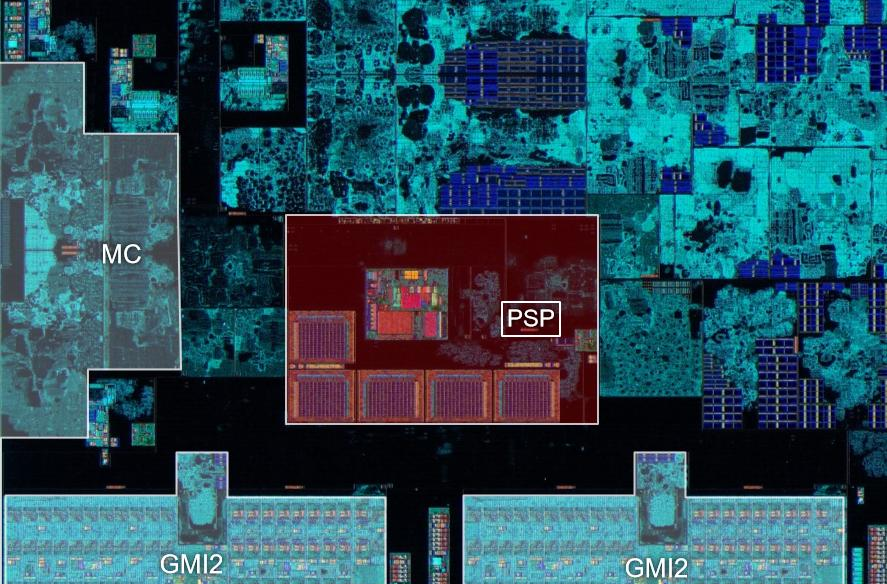
\includegraphics[width=0.9\textwidth]{figures/matisse-zen2.png}
    \caption{Fotografia di del chip \acrshort{amd} Matisse Zen2, con enfasi sul \acrshort{psp}. Crediti: Fritzchens Fritz.}
    \label{fig:matisse-zen2}
\end{figure}

Tali caratteristiche potrebbero sollevare preoccupazioni riguardo la possibile esposizione di chiavi e altre informazioni sensibili attraverso vulnerabilità come quelle scoperte in attacchi noti come quello del "glitch" PSPReverse. Nonostante queste potenzialità, la tecnologia \acrshort{psp} si distingue anche per la sua applicazione in ambito di protezione avanzata dei dati e di isolamento sicuro, ma la sua natura chiusa e la mancata documentazione sollevano interrogativi circa la trasparenza e il controllo su tali sistemi.

\subsection{Considerazioni}\label{subsec:considerazioni_txt_psp}

Sia Intel \acrshort{txt} che \acrshort{amd} \acrshort{psp} operano su principi simili, ovvero fornire una protezione a livello hardware contro la manipolazione del sistema e garantire che solo codice fidato venga eseguito. La differenza principale risiede nell'implementazione e nelle capacità specifiche di ciascuna piattaforma. Intel \acrshort{txt} si integra strettamente con il \acrshort{tpm} per misurare e validare l'integrità del sistema fin dall'avvio, mentre \acrshort{amd} \acrshort{psp} agisce come un'unità di sicurezza indipendente che gestisce in modo autonomo la protezione del sistema, senza fare affidamento diretto su un \acrshort{tpm}, ma su un’implementazione \acrshort{ftpm} propria.

Nel complesso, entrambe le tecnologie offrono solide basi per la creazione di sistemi sicuri. Queste tecnologie sono essenziali nell'evoluzione dei sistemi Trusted Processing Modules, poiché aumentano la resistenza contro minacce sia a livello di software che hardware.

\subsection{\texorpdfstring{\acrshort{amd} \acrshort{ftpm} stuttering}{AMD fTPM stuttering}}\label{subsec:amd_ftpm_stuttering}

Il problema di stuttering legato a \acrshort{ftpm} di \acrshort{amd} è stato rilevato per la prima volta su Windows nel 2022, quando gli utenti hanno notato blocchi casuali del sistema, non dipendenti dal carico di lavoro.

A partire dal kernel Linux 6.1, l'implementazione del \acrshort{ftpm} di \acrshort{amd} è stato abilitato per la generazione di numeri casuali tramite il modulo hardware \acrshort{rng}, impiegato per scopi di sicurezza. In particolare, quando un sistema è equipaggiato con un'unità \acrshort{ftpm} di \acrshort{amd}, il kernel utilizza automaticamente questa risorsa per gestire le operazioni che richiedono numeri casuali, con l'obiettivo di migliorare la sicurezza complessiva del sistema.

Tuttavia, questa implementazione ha causato problemi su alcune piattaforme, in particolare con processori \acrshort{amd} Ryzen, dove l’interazione tra \acrshort{ftpm} e il sistema di generazione dei numeri casuali ha provocato freeze intermittenti noti come stuttering, che si manifestavano in modo casuale durante l'utilizzo del computer. Questo comportamento è stato identificato come un bug legato al \acrshort{ftpm} e al modulo \acrshort{rng}.

Il rilascio di patch per risolvere il problema sono state precedute da accese discussioni nella comunità Linux. Nel luglio 2023, Linus Torvalds ha criticato aspramente l'implementazione, definendola "stupida" e suggerendo di disabilitarla per la generazione di numeri casuali. Una patch introdotta nel kernel 6.3 ha disabilitato \acrshort{ftpm} per l'\acrshort{rng} su sistemi problematici, ma il problema è riemerso anche con il kernel 6.4. La soluzione attuale prevede la disattivazione del supporto \acrshort{tpm} \acrshort{rng} per tutti i \acrshort{ftpm}, riducendo il problema senza eliminarlo completamente su alcune piattaforme.

Questo dibattito evidenzia le sfide nell'implementazione di soluzioni di sicurezza hardware e l'importanza di garantire che tali funzionalità non compromettano l'esperienza dell'utente finale.

\subsection{\texorpdfstring{Attacco faul\acrshort{tpm} \acrshort{amd}}{Attacco faulTPM AMD}}\label{subsec:attacco_faultpm_amd}

Un gruppo di ricercatori dell'Università Tecnica di Berlino ha recentemente individuato una vulnerabilità in alcune implementazioni \acrshort{ftpm}. Il loro studio dimostra come sia possibile compromettere \acrshort{psp} attraverso un attacco basato sull'iniezione di guasti (fault injection) tramite manipolazione della tensione in ingresso.

L’attacco sfrutta l'alterazione controllata della tensione di alimentazione del \acrshort{psp} all'interno delle architetture Zen 2 e Zen 3. Attraverso questa tecnica -- denominata faultTPM, i ricercatori sono riusciti a estrarre il "segreto" univoco di \acrshort{ftpm}, rendendo possibile la decodifica di tutti gli oggetti associati al modulo di sicurezza, e persino l’elusione di BitLocker di Windows.

Il team ha utilizzato strumenti economici e ha pubblicato sia codice che le specifiche dell’hardware impiegato su GitHub. L'attacco richiede ore di lavoro, accesso fisico al dispositivo e competenze avanzate, rendendolo difficile da eseguire su larga scala.

Nonostante la gravità della scoperta, il rischio per gli utenti è limitato, poiché l'attacco richiede accesso fisico. Tuttavia, una vulnerabilità così profonda solleva preoccupazioni significative. Rispetto ad altri attacchi side-channel, faultTPM rappresenta un avanzamento notevole, poiché consente di compromettere completamente il \acrshort{tpm} senza bypassare misure software complesse.

\acrshort{amd} non ha ancora rilasciato una soluzione definitiva, e il problema potrebbe non essere risolvibile con semplici aggiornamenti firmware. Possibili contromisure includono l'adozione di moduli \acrshort{tpm} hardware dedicati o una revisione architetturale. Al momento, gli utenti più esposti sono quelli che operano in ambienti ad alta sicurezza, dove l'accesso fisico ai dispositivi è una minaccia concreta.

\clearpage
\section{\texorpdfstring{Nota sull'\acrshort{iot}}{Nota sull'IoT}}\label{sec:nota_iot}

L’Internet of Things (\acrshort{iot}) ha portato a una crescente necessità di soluzioni di sicurezza integrate, poiché i dispositivi connessi operano spesso in ambienti esposti che necessitano di isolamento per le operazioni sensibili. In questo contesto, il Trusted Computing gioca un ruolo cruciale.

I \acrshort{tpm}, inizialmente sviluppati per i \acrshort{pc}, si stanno evolvendo per soddisfare le esigenze dei \acrshort{soc} e dei dispositivi embedded. Soluzioni integrate, come \acrshort{ftpm} e \acrshort{dtpm}, permettono di implementare funzionalità di sicurezza direttamente nei processori, riducendo l'esposizione dei bus di comunicazione e abbattendo i costi hardware.

Storicamente, i \acrshort{soc} \acrshort{arm} hanno trovato una maggiore diffusione nei dispositivi mobili, come smartphone e tablet, e, di conseguenza, i sistemi TrustZone non hanno generalmente impiegato un \acrshort{tpm} hardware separato. Considerando che il futuro dell'Internet of Things (\acrshort{iot}) sarà probabilmente dominato da architetture \acrshort{arm} anziché da x86 o x64, l'adoption di soluzioni basate su TrustZone potrebbe risultare ancora più rilevante per garantire la sicurezza e l'affidabilità dei dispositivi connessi. Tuttavia, è importante considerare che i controllori generalmente utilizzati nei sistemi \acrshort{iot} non possiedono elevate capacità prestazionali; pertanto, le funzionalità di sicurezza devono essere progettate in modo da non compromettere l'usabilità e la correttezza operativa del dispositivo.